\documentclass{article}
\usepackage{tikz}
\usetikzlibrary{positioning, arrows.meta}

\tikzset{
    block/.style={draw, thick, text width=7em, minimum height=3em, align=center},
    arrow/.style={thick, ->, >=Latex},
}

\begin{document}

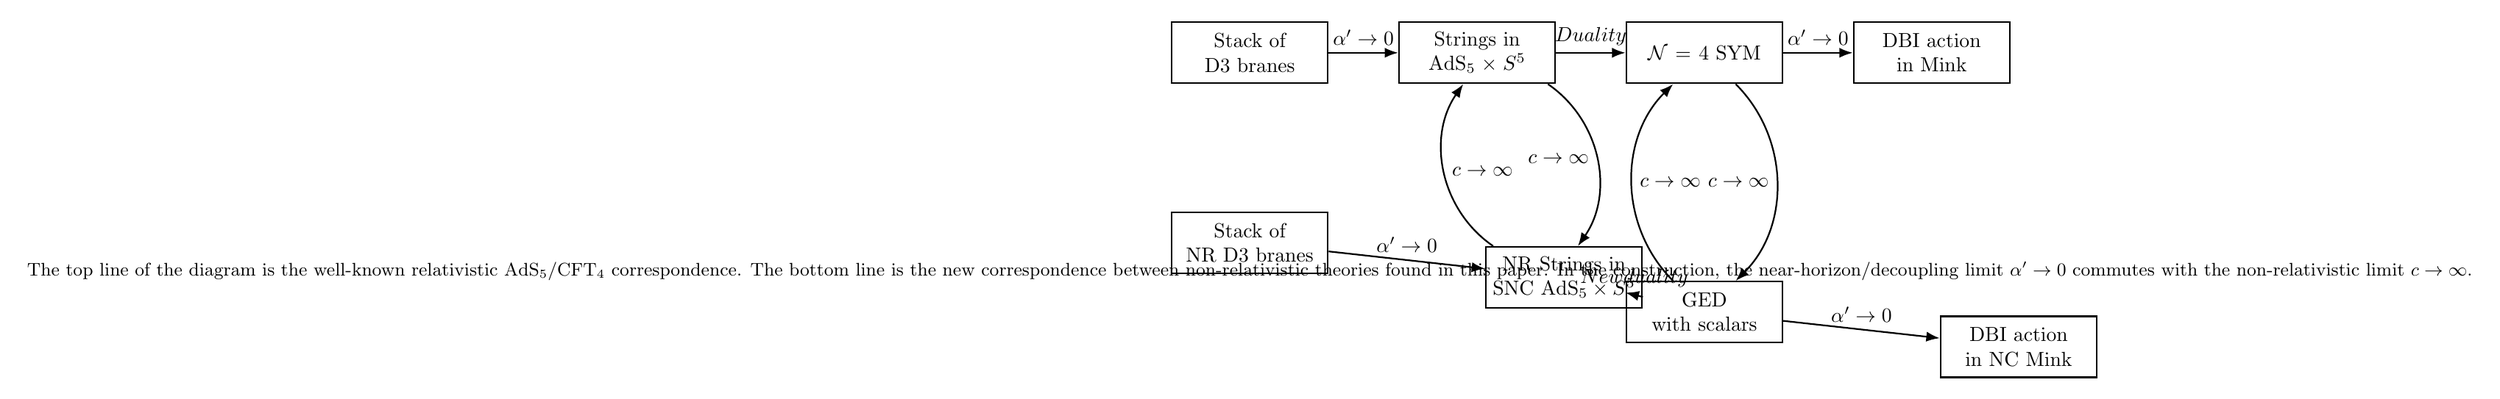
\begin{tikzpicture}[node distance=1.2cm]
    
    % Top line: relativistic AdS/CFT correspondence
    \node[block] (top1) {Stack of \\ D3 branes};
    \node[block, right=of top1] (top2) {Strings in \\ AdS${}_5 \times S^5$};
    \node[block, right=of top2] (top3) {$\mathcal{N}=4$ SYM};
    \node[block, right=of top3] (top4) {DBI action \\ in Mink};
    
    % Arrows for the top line
    \draw[arrow] (top1) -- node[midway, above]{$\alpha' \to 0$} (top2);
    \draw[arrow] (top2) -- node[midway, above]{$\text{Duality}$} (top3);
    \draw[arrow] (top3) -- node[midway, above]{$\alpha' \to 0$} (top4);
    
    % Bottom line: non-relativistic AdS/CFT correspondence
    \node[block, below=of top1, yshift=-1cm] (bottom1) {Stack of \\ NR D3 branes};
    \node[block, right=of bottom1, xshift=1.5cm, yshift=-0.6cm] (bottom2) {NR Strings in \\ SNC AdS${}_5 \times S^5$};
    \node[block, right=of bottom2, xshift=-1.5cm, yshift=-0.6cm] (bottom3) {GED \\ with scalars};
    \node[block, right=of bottom3, xshift=1.5cm, yshift=-0.6cm] (bottom4) {DBI action \\ in NC Mink};
    
    % Arrows for the bottom line
    \draw[arrow] (bottom1) -- node[midway, above]{$\alpha' \to 0$} (bottom2);
    \draw[arrow] (bottom2) -- node[midway, above]{$\text{New duality}$} (bottom3);
    \draw[arrow] (bottom3) -- node[midway, above]{$\alpha' \to 0$} (bottom4);
    
    % Arrows connecting the two lines
    \draw[arrow] (top2) edge[bend left=45] node[left]{$c \to \infty$} (bottom2);
    \draw[arrow] (bottom2) edge[bend left=45] node[right]{$c \to \infty$} (top2);
    \draw[arrow] (top3) edge[bend left=45] node[left]{$c \to \infty$} (bottom3);
    \draw[arrow] (bottom3) edge[bend left=45] node[right]{$c \to \infty$} (top3);
    
    % Annotations
    \node[below=0.2cm of top1 |- bottom1, font=\small] {The top line of the diagram is the well-known relativistic AdS${}_{5}$/CFT${}_{4}$ correspondence. The bottom line is the new correspondence between non-relativistic theories found in this paper. In the construction, the near-horizon/decoupling limit $\alpha'\to 0$ commutes with the non-relativistic limit $c\to \infty$.};
    
\end{tikzpicture}

\end{document}